\chapter{THE STANDARD MODEL AND SUPERSYMMETRY}
\label{chap:theory}

\section{The standard model of particle physics}
\label{sec:StandardModel}
The standard model (SM) of particle physics is a non-Abelian gauge theory that describes elementary particles and their allowed interactions
The first piece of the standard model was developed in 1961 (XX references! XX) with the unification of the electromagnetic and weak interactions. 
The Higgs mechanism was later incorporated into the standard model in 1967 (XX cite XX), and 
the standard model took on the form we know today with the inclusion of the strong force and quantum chromodynamics (QCD) in the 1970's (XX cite XX).
The standard model is incredibly successful, and it has made absurdly precise predictions that have held up to experimental scrutiny. 

The standard model is a Lorentz-invariant quantum field theory. The symmetry group of the standard model is 
\begin{equation}
G_{SM} = SU(3)_C \otimes SU(2)_L \otimes SU(1)_\Upsilon
\label{equ:symm}
\end{equation}
where $SU(3)_C$ is responsible for mixing the 3 \textit{colors} of quarks and antiquarks, $SU(2)_L$ represents \textit{weak isospin}, and $U(1)_\Upsilon$ couples to the \textit{weak hypercharge $\Upsilon$}. The combination $SU(2)_L \otimes SU(1)_\Upsilon$ corresponds to the electroweak interactions. 

%%%%%%%%%%%%%%%%%%%%%%%%%%%%%%%%%%%%%%%
\subsection{Particle content of the standard model}
\label{sec:SMparts}
The fields in the SM are identified by their representation in the symmetry group of Equation~\ref{equ:symm}. These are listed for the SM fermions in Table~\ref{tab:fermions} and for the gauge bosons in Table~\ref{tab:bosons}. There are three generations of quarks and three generations of leptons in the SM. The quarks are in a non-trivial representation of all three SM symmetries, and therefore interact via the strong, weak, and electromagnetic interactions. The three ``up-type" quarks are the up quark $u$, the charm quark $c$, and the top quark $t$. The three ``down-type" quarks are the down quark $d$, the strange quark $s$, and the bottom quark $b$. 

The three generations of leptons include the electron $e$, muon $\mu$, and tau $\tau$ and the corresponding neutrinos. In the SM, the neutrinos are massless, even though it has been experimentally established that at least two of the neutrinos must have non-zero mass XX citeXX. The electron, muon and tau particles participate in the weak interaction and the electromagnetic interaction, but the neutrinos, being electromagnetically neutral, only participate in the weak interaction. 

As can be seen in Table~\ref{tab:fermions}, the weak interaction does not respect parity. The left-handed quarks and leptons belong to $SU(2)_L$ doublets, whereas the right-handed quarks and leptons form $SU(2)_L$ singlets.
%right-handed leptons form singlets. If right-handed neutrinos exist, they are sterile and we have no evidence (can't have evidence?) for them
%Dirac spinor $\Psi$ and conjugate $\bar{\Psi}$ are equivalent to two left-handed Weyl spinors ($\chi$ and $\tilde{\chi}$)
%and their right-handed conjugates ($\chi^\dagger$ and $\tilde{\chi}^\dagger$).Tilde = anti

\begin{table}[ht]
    \caption{FERMIONS IN THE STANDARD MODEL}
    \centering
    \begin{tabular}{|c|c|c|c|}
    \hline
    \hline
    Name  & Symbol & $SU(3)_C,~SU(2)_L,~U(1)_\Upsilon $\\
  	  \hline
           \hline    
quarks        & ($u_L~d_L$)     & (\textbf{3}, \textbf{2}, $\frac{1}{6}$) \\
(3 families) & $u_R^\dagger$ & ($\bar{\textbf{3}}$, \textbf{1}, $-\frac{2}{3}$) \\
                   & $d_R^\dagger$ & ($\bar{\textbf{3}}$, \textbf{1}, $\frac{1}{3}$) \\
                   \hline
leptons       & ($\nu~e_L$)      &  (\textbf{1}, \textbf{2}, $-\frac{1}{2}$) \\
(3 families) & $e_R^\dagger$ &  (\textbf{1}, \textbf{1}, 1) \\
           \hline
           \hline
    \end{tabular}
    \label{tab:fermions}
%    \justify{Fermions in the standard model. }
\end{table}

%%%%%%%%%%%%%%%%%%%%%%%%%%%%%%%%%%%%%%%

The gauge bosons are responsible for mediating the interactions between the fermions. Before electroweak symmetry breaking (EWSB), the three gauge bosons of $SU(2)_L$ are the $W^+,~W^-,$ and $W^0$, and the $U(1)_\Upsilon$ gauge boson is the $B$ boson. After EWSB, the $W^+$ and $W^-$ bosons gain a mass, and the $W_0$ and $B$ bosons mix to form the massive $Z$ boson and the massless photon $\gamma$. EWSB will be described in more detail in Section~\ref{sec:EWSB}.

For the strong force $SU(3)_C$, the gauge bosons are the gluons. Processes involving the interactions of quarks and gluons are referred to as QCD processes. The QCD interaction is different from the electroweak interactions in that the strong force grows in strength at larger distances. This leads to the phenomenon of \textit{confinement}: at low energies and large distances (greater than ~1 GeV$^{-1}$), we cannot identify individual quarks or gluons. Instead, these particles can only be found in $SU(3)_C$ singlets, typically either mesons ($q\bar{q}$) or baryons ($qqq$ or $\bar{q}\bar{q}\bar{q}$). 

\begin{table}[ht]
    \caption{GAUGE BOSONS IN THE STANDARD MODEL}
    \centering
    \begin{tabular}{|c|c|c|c|}
    \hline
    \hline
    Name  & Symbol & $SU(3)_C,~SU(2)_L,~U(1)_\Upsilon $\\
  	  \hline
           \hline    
gluon         & $g$   & (\textbf{8}, \textbf{1}, 0) \\
\hline
$W$ bosons & $W^\pm,~W^0$ & (\textbf{1}, \textbf{3}, 0) \\
\hline
$B$ boson & $B^0$ & (\textbf{1}, \textbf{1}, 0) \\
           \hline
           \hline
    \end{tabular}
    \label{tab:bosons}
    \justify{Gauge bosons in the standard model before electroweak symmetry breaking. }
\end{table}

%%%%%%%%%%%%%%%%%%%%%%%%%%%%%%%%%%%%%%%

Finally, the only particle not included in Table~\ref{tab:fermions} or \ref{tab:bosons} is the Higgs boson. The Higgs boson was discovered by the CMS and ATLAS collaborations in 2012 XX cite XX, and is responsible for electroweak symmetry breaking (EWSB), which will be described in Section~\ref{sec:EWSB}. It is the only fundamental scalar in the SM and has a mass of approximately 125 GeV. The Higgs boson is in the  (\textbf{1}, \textbf{2}, $+\frac{1}{2}$) representation of $G_{SM}$, and is therefore uncharged under the strong and electromagnetic interactions. 

Figure~\ref{fig:SMint} summarizes the SM particles and their allowed interactions.

\begin{figure*}[htbp]
    \centering
    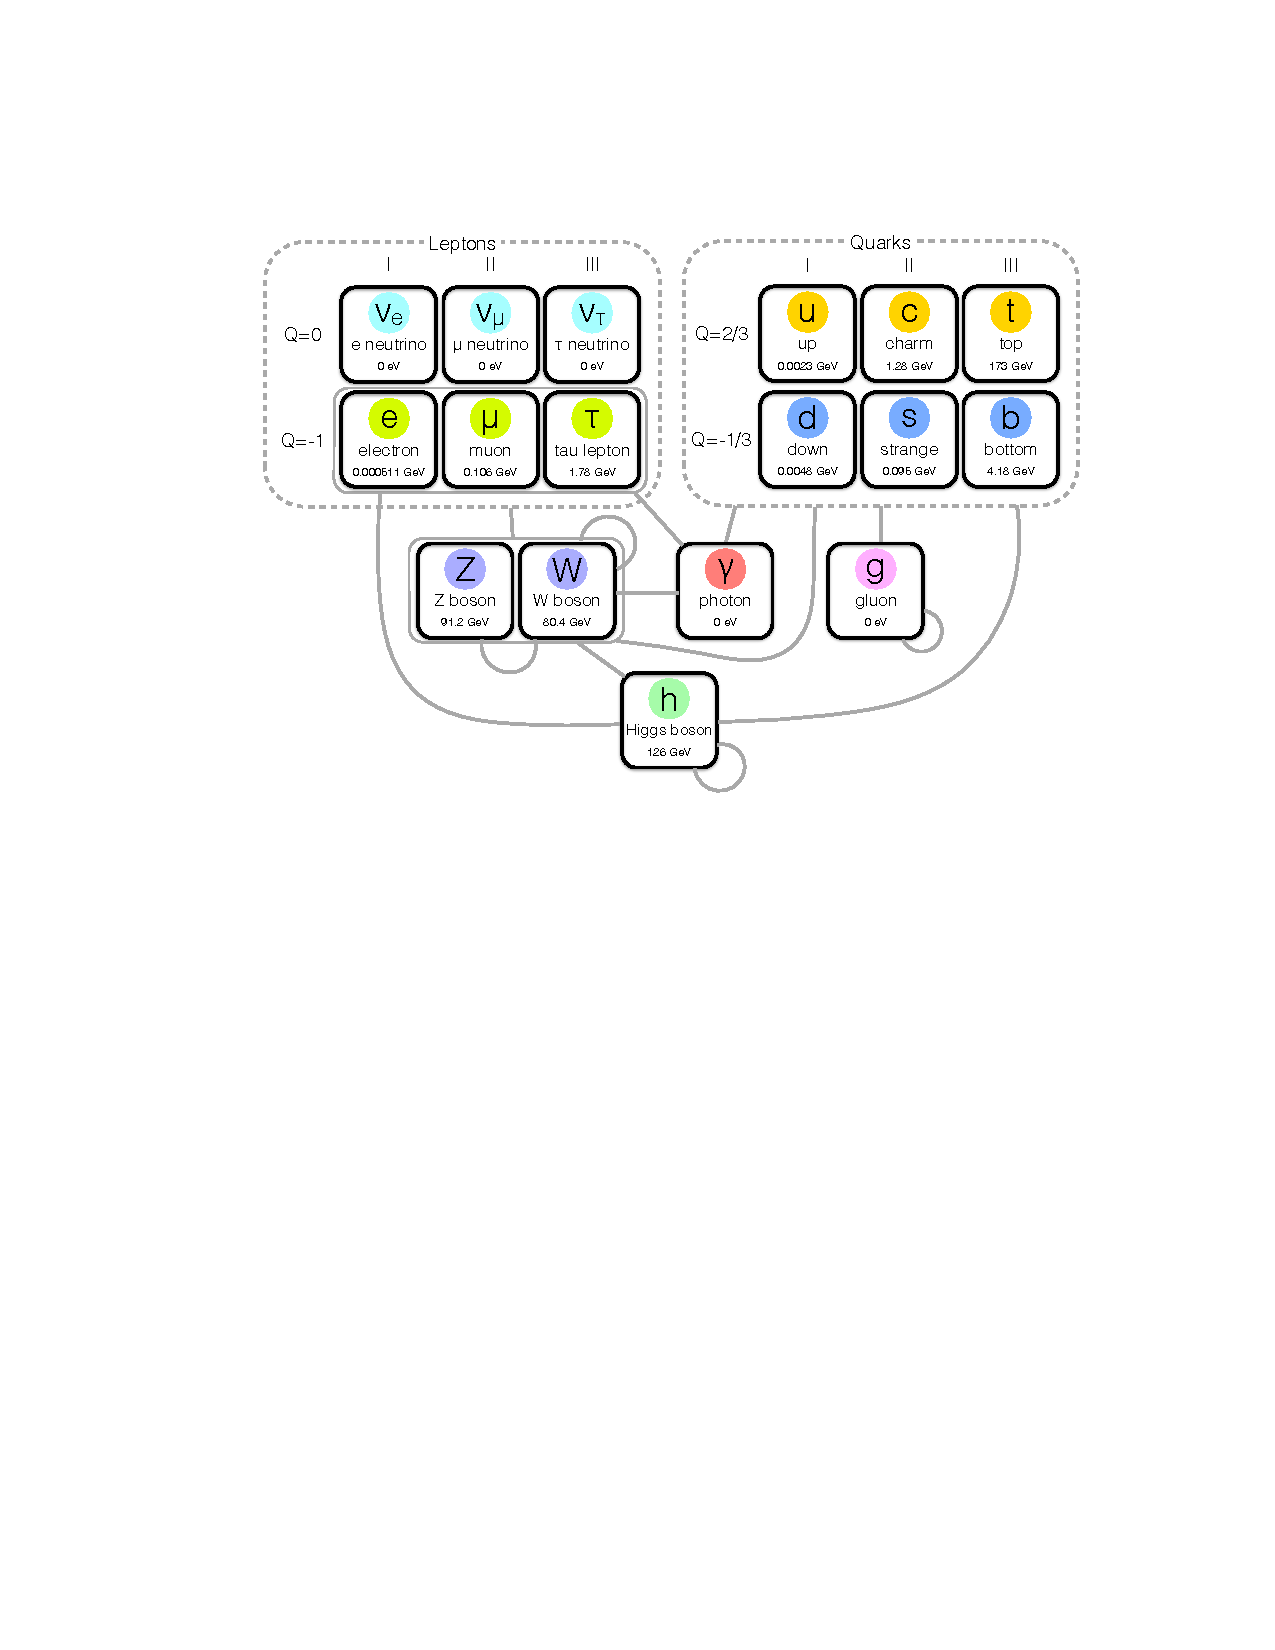
\includegraphics[width=\textwidth]{Figures/Theory/SM_Interactions.pdf}
    \caption{Particle content of the standard model. Allowed interactions are indicated with gray lines between particles or particle groups. The mass of each particle is listed underneath its symbol and name. The electric charge Q of the leptons and quarks is also indicated. Particles connected to themselves can have self-interactions.
    Reprinted from Reference~\cite{Yutaro}.}
    \label{fig:SMint}
\end{figure*}

%%%%%%%%%%%%%%%%%%%%%%%%%%%%%%%%%%%%%%%
%%%%%%%%%%%%%%%%%%%%%%%%%%%%%%%%%%%%%%%

\subsection{Electroweak symmetry breaking}
\label{sec:EWSB}
Electroweak symmetry breaking is a crucial feature of the standard model. The electroweak symmetry is spontaneously broken through the Higgs mechanism. 
The scalar potential of the complex Higgs field $H$ is
\begin{equation}
V(H^\dagger H) =  \mu^2(H^\dagger H) + \lambda(H^\dagger H)^2. 
\label{equ:HiggsV}
\end{equation}

The mass parameter $\mu^2$ is negative, which means that the vacuum expectation value (vev) of the Higgs (written as $\langle H \rangle$ or $v$) is non-zero. The Higgs potential is illustrated in Figure~\ref{fig:HiggsV}. Spontaneous symmetry breaking occurs when the value of the Higgs field ``rolls" from the unstable position at the origin and comes to rest at the stable minima:
\begin{equation}
\langle H \rangle= v = \sqrt{\frac{-\mu^2}{2\lambda}}.
\end{equation}

During EWSB, three of the four degrees of freedom in the Higgs complex scalar doublet get ``eaten" to give mass to the $W^\pm$ and $Z$ bosons. The last degree of freedom becomes the scalar Higgs boson. The mass $m_H$ of the Higgs boson can be written in terms of the parameters $\mu$ and $\lambda$: 
\begin{equation}
m_H = \sqrt{-\mu^2} = v\sqrt{2\lambda} = 125 \mathrm{GeV}.
\label{equ:HiggsMass}
\end{equation}

The remaining symmetry is $U(1)_{\textrm{EM}}$, which corresponds to the electromagnetic interaction. The massless photon is the gauge boson of $U(1)_{\textrm{EM}}$ and couples to the electric charge Q: 
\begin{equation}
Q = T^3 + \Upsilon
\end{equation}
where $\Upsilon$ is the weak hypercharge and $T^3$ is the isospin. The short-range weak interactions are mediated by the $W^\pm$ and $Z$ bosons, and the photon mediates the long-range electromagnetic interactions.

%%%%%%%%%%%%%%%%%%%%%%%%%%%%%%%%%%%%%%%
\subsection{Limitations of the standard model}
\label{sec:SMweakness}
It is undeniable that the standard model has been a huge triumph of modern physics. However, there are known limitations. These fall into two categories: experimentally-established phenomena which are not incorporated into the standard model, and unsettling questions that the standard model cannot answer but which perhaps would be explained by some more fundamental theory. 

Neutrino masses---an example of the first category---have already been mentioned. The prevalence of matter over antimatter (CP violation) is another observed contradiction to the standard model as it exists today. The only SM source of CP violation is quark mixing, which is not nearly large enough to explain why the universe is more than just a bath of radiation from the annihilation of particles and antiparticles. 

The existence of dark matter also falls into the first category. A wealth of evidence, including galaxy cluster velocity dispersions, gravitational lensing studies, and measurements of the Cosmic Microwave Background, indicates that approximately 25\% of the energy budget of the universe is contained in dark matter (see Reference~\cite{DarkMatterReview} for a review). We know that dark matter interacts gravitationally, and stringent limits have been placed on the strength of its other interactions. However, so far there is no conclusive evidence as to the nature of dark matter.

The second category includes questions about why the 19 free parameters in the standard model have the values that they do. For instance, it could be seen as unsettling that the masses of the particles in Figure~\ref{fig:SMint} cover such a large range, from $m_e = 0.000511$ GeV to $m_t = 173$ GeV. The problem of ``fine-tuning" is often discussed in this context. A theory is said to be fine-tuned if several free parameters have to take on precise values and interact in a convenient way in order to explain the observed results. While nothing is inherently wrong with a fine-tuning, it is a very unsatisfying way to solve a problem.

The hierarchy problem is a particularly worrisome fine-tuning problem. As already stated in Equation~\ref{equ:HiggsMass}, the mass parameter $\mu$ in the Higgs potential can be written in terms $v$ and $\lambda$, where the vev $v$ has been measured to be \~174 Gev. What was not mentioned, however, is that there are huge quantum corrections to $\mu^2$ from loop diagrams. 

%%%%%%%%%%%%%%%%%%%%%%%%%%%%%%%%%%%%%%%

%12 vector fields (spin 1)- gauge fields of the SU(3) x SU(2) x U(1)
%45 Weyl fermion fields: [21 Dirac spinors  (3 colors x 6 quarks) + 3 charged leptons] x2 to get to  weyl+ 3 neutrinos
%complex doublet H of scalar fields

%Left-handed Weyl components of quark Dirac spinors form 9 doublets of $SU(2)_W$ (3 flavor doublets per 3 color)
%Right-handed Weyl components of quark Dirac spinors are 18 $SU(2)_W$ singlets. Weak interactions can break parity

%Left-handed leptons form 3 $SU(2)_W$ doublets 
%right-handed leptons form singlets. If right-handed neutrinos exist, they are sterile and we have no evidence (can't have evidence?) for them
%Dirac spinor $\Psi$ and conjugate $\bar{\Psi}$ are equivalent to two left-handed Weyl spinors ($\chi$ and $\tilde{\chi}$)
%and their right-handed conjugates ($\chi^\dagger$ and $\tilde{\chi}^\dagger$).Tilde = anti


%http://bolvan.ph.utexas.edu/~vadim/Classes/2011f/SM.pdf

\section{Supersymmetry}
\label{sec:SUSY}

Motivations:
Higgs mass, contributions 
Hierarchy problem 

\begin{table}[ht]
    \caption{CHIRAL SUPERMULTIPLETS IN MSSM}
    \centering
    \begin{tabular}{|c|c|c|c|c|}
    \hline
    \hline
    \multicolumn{2}{|c|}{Names} & Spin 0 & Spin 1/2 &$SU(3)_C,~SU(2)_L,~U(1)_\Upsilon $\\
  	  \hline
           \hline    
squarks, quarks  & Q & ($\tilde{u}_L~\tilde{d}_L$) & ($u_L~d_L$)  & (\textbf{3}, \textbf{2}, $\frac{1}{6}$) \\
(3 families) & $\bar{u}$ & $\tilde{u}_R^\ast$ & $u_R^\dagger$ & ($\bar{\textbf{3}}$, \textbf{1}, $-\frac{2}{3}$) \\
                   & $\bar{d}$ & $\tilde{d}_R^*$     & $d_R^\dagger$ & ($\bar{\textbf{3}}$, \textbf{1}, $\frac{1}{3}$) \\
                   \hline
sleptons, leptons  & $L$ & ($\tilde{\nu}~\tilde{e}_L$) & ($\nu~e_L$)      &  (\textbf{1}, \textbf{2}, $-\frac{1}{2}$) \\
(3 families) & $\bar{e}$ & $\tilde{e}_R^\ast$  & $e_R^\dagger$ &  (\textbf{1}, \textbf{1}, 1) \\
\hline
Higgs, higgsinos & $H_u$  & ($H_u^+ ~ H_u^0$) & ($\tilde{H}_u^+ ~ \tilde{H}_u^0$) & ($\textbf{1}$, \textbf{2}, $+\frac{1}{2}$) \\
                           & $H_d$  & ($H_d^0 ~ H_d^-$) & ($\tilde{H}_d^0 ~ \tilde{H}_d^-$) & ($\textbf{1}$, \textbf{2}, $-\frac{1}{2}$) \\
           \hline
           \hline
    \end{tabular}
    \label{tab:SUSY_fermions}
    \justify{Reprinted from Reference~\cite{SUSYprimer}.}
\end{table}

\section{Gauge-mediated supersymmetry breaking}
\label{sec:gmsb}

